%*******************************************************************************
%*********************************** First Chapter *****************************
%*******************************************************************************


\chapter{Literature Survey}  %Title of the First Chapter


\graphicspath{{Figs/}}


%********************************** %First Section  **************************************

\section{Abstract} %Section - 1.1 
Abstract about machine learning and pattern recognition.
Machine learning has had many successes in recent years in many different fields. However particle physics has been slow to adapt, with multivariate analysis techniques only seeing use as simple classifiers of signal and background for example. VELO pattern recognition is the process that takes hits in the VELO detector, and constructs tracks for use in physics analysis. Required speed ups for Run III of LHCb in 2021 mean that a new approach to software is needed due to a vast increase in data rate and limited resources. Machine learning techniques such as neural networks could satisfy the need for efficient and fast VELO pattern recognition.

%********************************** %First Section  **************************************

\section{Introduction} %Section - 1.1 
Introduction to machine learning and pattern recognition.

%********************************** % Third Section  *************************************

\section{A brief history of Machine Learning}  %Section - 1.3
Machine learning is not a new idea, but has seen a great increase in popularity in recent years. The history of machine learning is almost as old as computing itself, it was in 1950 that Alan Turing published \textit{Computing Machinery and Intelligence} \cite{TURING1950I.COMPUTINGINTELLIGENCE}, in which he laid out his ideas about the ability of machines to think and learn. Turing's criteria have since become known as the 'Turing Test'. Initial research into machine learning took the form of mimicking the neurons in the brain, and it was in 1957 that Frank Rosenblatt invented the \textit{perceptron}. A perceptron is an algorithm for binary linear classification see figure \ref{fig:SingleLayerPerceptron}. It can decide if an object is one of two classes and can draw a straight line to differentiate populations of objects shown in figure \ref{fig:Perceptron_example}.  

\begin{figure}[h] % h for here in document
\centering
\begin{subfigure}[t]{0.45\textwidth}
\centering
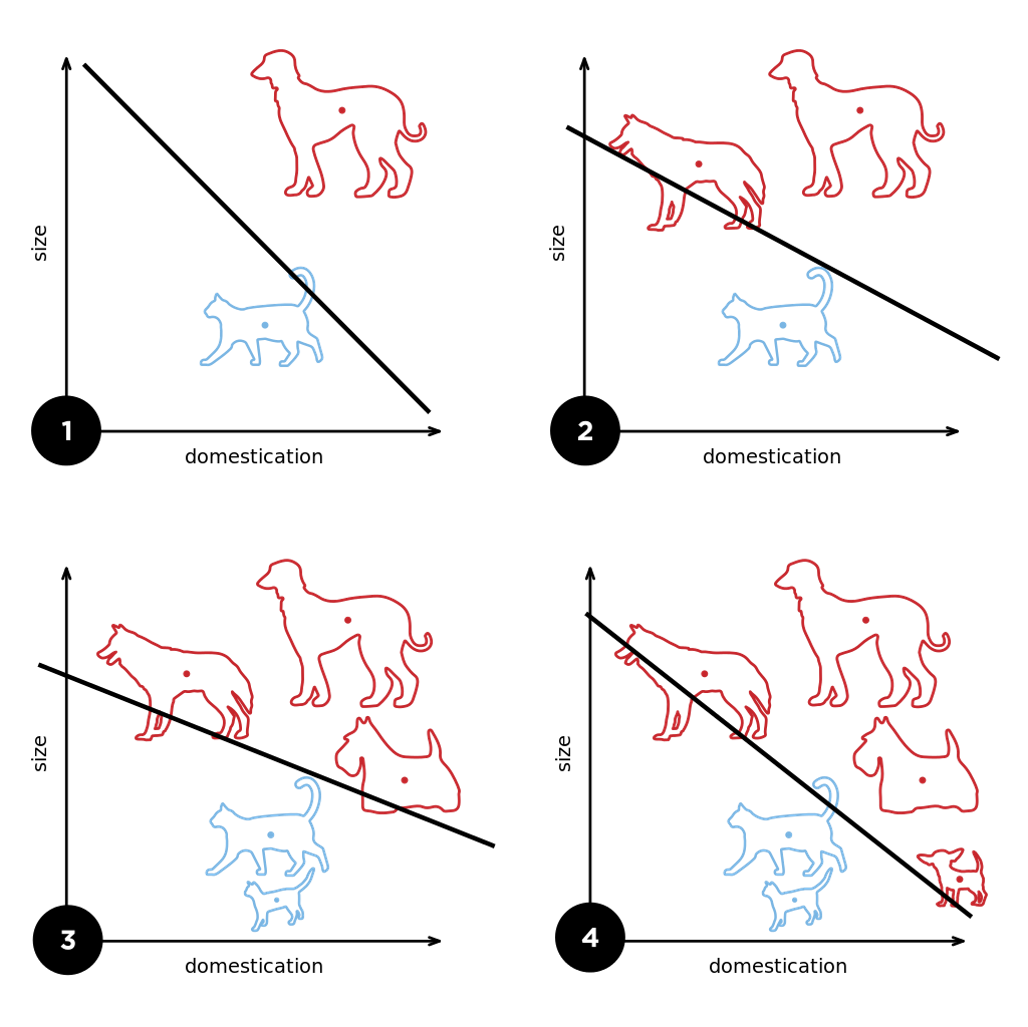
\includegraphics[width=\textwidth]{Perceptron_example}
\caption{A diagram of a perceptron learning to change its linear boundary as more training data is added. In this it is classifying whether an animal is a cat or a dog depending on its size and level of domestication.} 
\label{fig:Perceptron_example} 
\end{subfigure}
~
\begin{subfigure}[t]{0.45\textwidth}
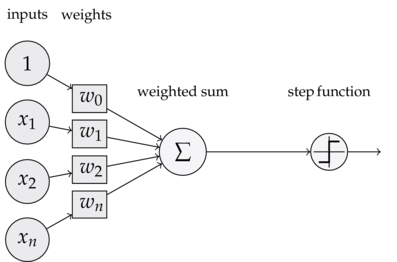
\includegraphics[width=\textwidth]{SingleLayerPerceptron}
\caption{Diagram of a single layer perceptron, as described by Rosenblatt. A feature vector is fed in and a weighted sum is made of the features. A step function is used as an activation to give the binary output of 0 or 1.} 
\label{fig:SingleLayerPerceptron}
\end{subfigure}
\end{figure}

Rosenblatt was highly optimistic about the abilities of the perceptron. However in 1969 Marvin Minsky and Seymour Papert published their book \textit{Perceptrons: an introduction to computational geometry} \cite{Minsky1969Perceptrons:Geometry} in which they proved mathematically that a single layer perceptron could not learn, for example, the XOR logic function. This controversial book signalled the start of the first 'dark age' of machine learning, however it was not to last long.\\
Machine learning research would rise again after the invention of \textit{back propagation}. Back propagation was a new method of learning developed by David Rumelhart, Geoffrey Hinton  and Ronald Williams and published in 1986 \cite{Rumelhart1986LearningErrors}. This paper introduced the idea of a network of 'hidden layers', unlike previous multilayer perceptrons these hidden layers had weights set by a back propagation algorithm, rather than by hand. The back propagation algorithms job was to tune the weights of neurons to reduce the difference between the network output and the desired output. This breakthrough allowed these 'neural networks' to learn non-linear functions, not possible with simple perceptrons. Further papers proved that neural networks could theoretically learn any non-linear function, given enough neurons \cite{Hornik1991ApproximationNetworks}. Early success was had with convolutional neural network used to identify handwritten digits \cite{LeCun1990HandwrittenNetwork}. However funding cuts, expensive systems and a long list of missed goals led an 'AI winter'. With many losing faith in artificial intelligence. This did not stop IBM, who in 1997 beat reigning world chess champion Garry Kasparov with their machine 'Deep Blue', and for the first time showed the capabilities of artificial intelligence. Deep Blue used massively parallel computing to calculate hundreds of millions of positions every second \cite{Campbell2002DeepBlue}. This brute force approach is not the same as other machine learning methods discussed.\\
It was not until the 'big data' revolution of the 21st century that machine learning was truly taken seriously. The mid 2000's saw a series of revolutionary papers that greatly improved the performance of neural networks. Greedy layerwise training was first proposed in 2006 \cite{Bengio2006GreedyNetworks}, as a way to initialise the weights of a neural network before the supervised learning stage. Random initialisation would often lead to poor final solutions. Increasing computing power meant that the power of neural network could finally be realised.

%********************************** %Fourth Section  *************************************

\section{Introduction to Deep Learning} %Section - 1.4
The deep neural network comprises of many hidden layers is the backbone of Deep learning. It has been demonstrated to very capable of image and sound classification, and many other 'big data' problems.

%********************************** %Fifth Section  *************************************

\section{VELO Track Reconstruction} %Section - 1.5
VELO track reconstruction is the name for a series of algorithms that takes hits in the VELO and returns tracks. These tracks are then used for physics analysis. This section will describe the known method for VELO upgrade track reconstruction \cite{Bird:1620453}.

\subsection{Definitions}
Define measurements, clusters, tracks, states etc. \cite{Hernando:1057515}

\subsection{Clustering}
Particles will often deposit energy in more than one pixel in each sensor. A group of pixels belonging to the same hit is known as a cluster. The number of pixels in a cluster is determined by the angle the particle passed through the sensor. A steeper angle will create larger clusters whilst shallower angles will create smaller clusters. Each pixel has a binary readout, meaning a cluster is represented by a small group of 1's in a large array of 0's. The clustering software looks for groups of up to 8 connected hits, these can be connected horizontally, vertically or diagonally.

\subsection{Pattern Recognition}
Clusters are stored with errors $\Delta$x and $\Delta$y. These errors are used for calculating weights for the track fit later in the process, and are approximated by $\Delta x = \Delta y = p/\sqrt{12}$ where $p$ is the size of each pixel.
The method of pattern recognition currently developed works as follows:
\begin{enumerate}
    \item Starting from the most downstream module (module with the largest $z$) pairs of unused clusters in the next upstream module are investigated. These cluster pairs must have track slopes $|dx/dz|<0.4$ and $|dy/dz|<0.4$. The restriction of track slopes is used so that only tracks that lead roughly towards the interaction point are looked at.
    \item Step 1 will produce a number of possible track seeds between every pair of adjacent modules, to determine which seed is correct each track seed is extrapolated to the next upstream module. A small window is drawn around each extrapolated hit in the 3rd module, if there are any clusters inside this window then this cluster will be added to the track.
    \item After this process is complete tracks that contain less than three clusters are rejected. Tracks with exactly three clusters must contain only unused clusters and pass a cut on the track $\chi^2$ from a least-squares fit. Tracks with more contain more than three clusters must at least 50\% unused clusters, if this is true then all clusters are added to the track and tagged as used.
    \item The next stage is to convert each temporary track to a \verb|Track::Velo| object. If the z-position at which the track is closest to the beam line is larger than the maximum z-position of any cluster then the track is labelled as a backward track, otherwise it is labelled as a forward track. The track is then fit using a Kalman filter with scattering. This method if fitting gives better impact parameter resolution than a standard straight line fit. The scattering per layer is approximated by
    $$\sigma_{MS}^{2}=a+b(t_{x}^{2}+t_{y}^{2})$$
    where $t_x$ and $t_y$ are the track slopes and $a$ and $b$ are parameters determined from Monte Carlo simulation.
    \item Finally track states are calculated for each track. A track state is simply an $x,y,z$ coordinate with errors on $x$ and $y$. Track states are calculated for each track at a z-position closest to the beam line and at the end of the VELO (defined as z=770mm).
\end{enumerate}
It is this step I will be trying to improve through the application of machine learning.

\subsection{Parallel method}
The current method is sequential, this means that each layer is looked at individually and tracks built from the outside of the VELO towards the interaction point. Parallel computing can offer large speed ups when a problem involves many small, independent calculations. An attempt to parallelise VELO upgrade pattern recognition has been made and will be described \cite{Ticse:1554078}. However this is not the only example \cite{Abba:1667587}.
\begin{enumerate}
    \item Instead of starting in the outermost module, all modules are looked at simultaneously. Firstly the algorithm finds all pairs of clusters (Tracklets) in given angular range.
    \item Information about each tracklet is stored. These are the slope in x and y $(dx,\ dy)$, and the projection to a plane beyond last velo layer, known as the \textit{e-plane} $(ex,\ ey)$. figure \ref{fig:SIMDVeloPR}
    
    \begin{figure}[h] % h for here in document
    \centering 
    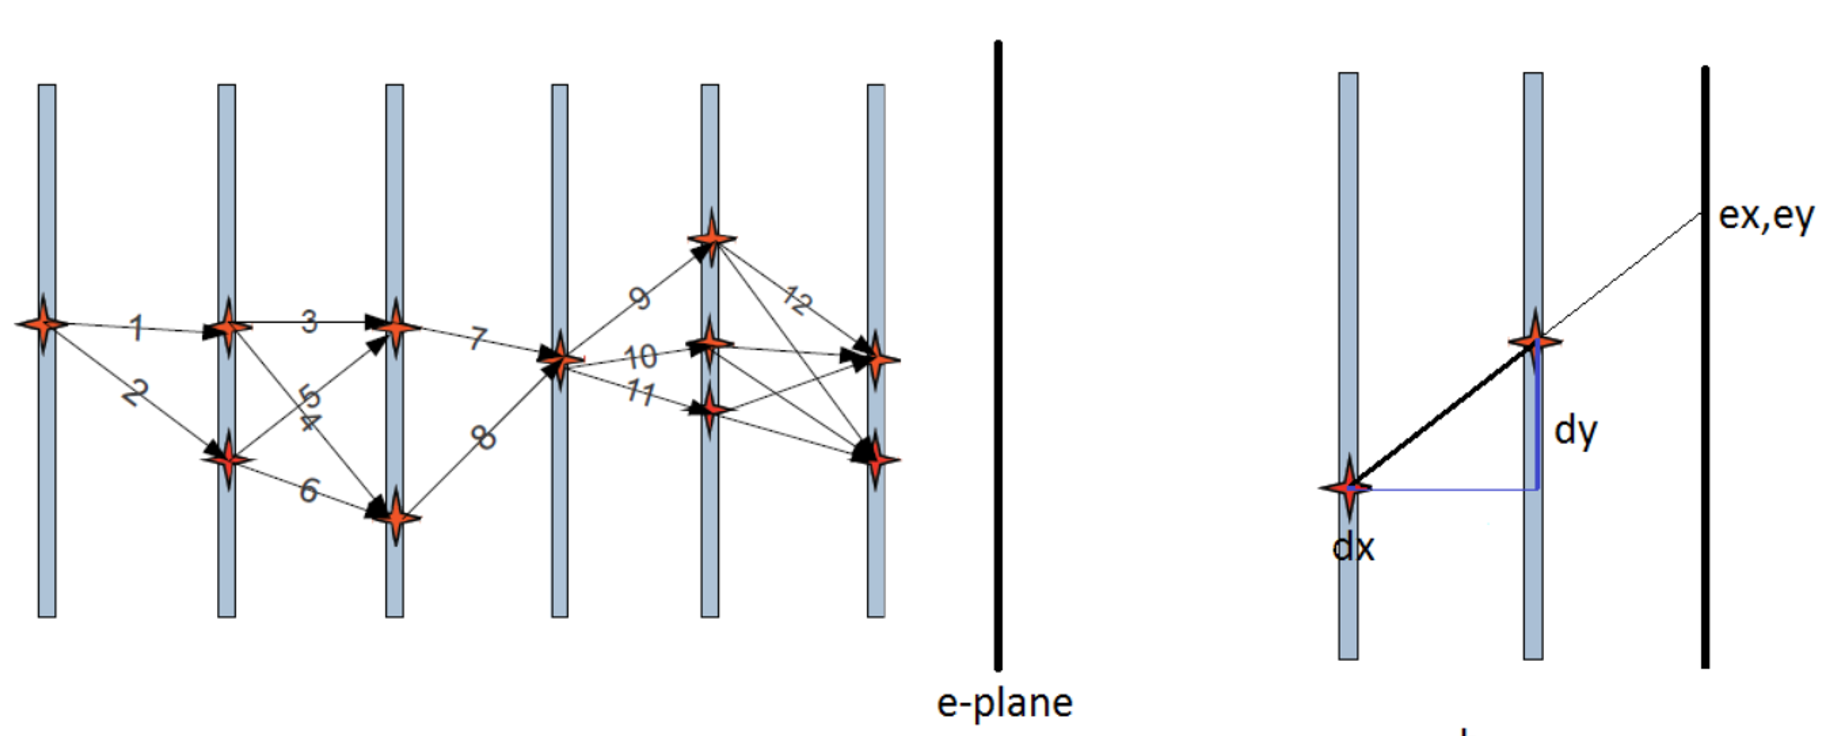
\includegraphics[width=\textwidth]{SIMDVeloPR}
    \caption{Diagram of tracklet formation and definition of parameters.} 
    \label{fig:SIMDVeloPR} 
    \end{figure}

    \item To connect tracklets into tracks calculate the gradient and projection distance for every pair of tracklets. As these distances are independent of each other these can be calculated  quickly in parallel. For each tracklet this will give a list of gradient and projection distances for all other tracklets between different modules. 
    \item Tracklets with similar gradient and projection distance should be part of same track. Groups of tracklets with small gradient and projection distances are probably in the same track. By defining a maximum distance between these distance tracklets can be grouped into tracks.
\end{enumerate}
This method was demonstrated to work well on low density data, with few clusters and tracks. With efficiency and purity up to 88\%. However with high cluster and track densities the efficiency and purity reduced significantly. Down to 55\% efficiency and 3\% purity.\\
Efficiency is defined as the number of correctly reconstructed tracks divided by the number of tracks. And purity is defined as ...\\
This method is not fully developed and has many areas in need of improvement. However it is still an interesting look into speeding up the pattern recognition system.


\subsection{Efficiency}
Monte Carlo simulation truth can be used to calculate the efficiency of this method. The efficiency is calculated by comparing the number of correctly reconstructed tracks to the number of reconstructible tracks from the MC. The following definitions are used by LHCb:

\begin{itemize}
    \item A track is reconstructible as a VELO track if there are clusters associated to it on three or more modules
    \item A track is reconstructible as a “long track” if it is reconstructible as a VELO track and, in addition, has at least one x and one “stereo” hit in each of the three downstream track seeding stations.
    \item A particle is considered reconstructed if at least 70\% of the measurements on a track are associated to this particle.
    \item A ghost track or fake track is a track which cannot be associated to any simulated particle.  If more than one reconstructed track is associated to a particle the extra tracks are counted as clone tracks.
    \item $\epsilon_{rec}=\frac{N_{correctly\ reconstructed}}{N_{reconstructible}}$
\end{itemize}
The method described above can achieve very high efficiency's of >99\%, more than that of the current VELO \cite{Collaboration:1624070}. However it is not optimised for speed.

